\chapter{Introduction}

\section{Statement of Purpose}

Recognizing activities in videos has become a hot topic over the last years in the computer vision community~\cite{ngiam2011multimodal}. The exponential growth of portable video cameras and online multimedia repositories, as well as recent advances in video coding, storage and computational resources have leaded research in the field towards new and more efficient solutions for organizing, understanding and retrieving video content.

Deep learning techniques have recently become the new state of the art in many computer vision tasks, such as image and object recognition in still images. While successful methodologies have been presented for image understanding, video content still presents additional challenges (e.g. motion, temporal consistency, ...)  that often cannot be bridged with still image recognition solutions.  

The purpose of this work is to face the challenges of video content analysis taking advantage of state-of-the-art deep learning techniques. The aim of this project is to offer a good framework to both classify and temporally localize activities on videos. To achieve this goal, the dataset used to fulfill this task will be the ActivityNet dataset \cite{caba2015activitynet}, which offers untrimmed videos which a huge variety of activities on it.

%Rather than focusing on activity classification on videos, the aim of this project is to offer a good framework to detect and localize activities on videos. To achieve this goal, the dataset used to fulfill this task will be the ActivityNet dataset \cite{caba2015activitynet}, which offers untrimmed videos which a huge variety of activities on it.

% AMAIA: I think that it is fine to say that you will both address activity classification and detection in your thesis, not just detection... DONE

In particular, this project's main contributions are:
\begin{itemize}
	\item The design and training of the architecture, which is based on 3D Convolutional features and Recurrent Neural Networks.
    \item The development and analysis of post processing techniques for classification and temporal localization
    \item The release of an open sourced package containing all the tools to reproduce the experiments, as well as the conversion of a state-of-the-art 3CD model from Caffe to Keras.
    
% REMOVED:    \item A framework to classify and localize activities on videos using deep learning techniques, more precisely using recurrent neural networks.
%    \item Develop techniques to process sequence output from Recurrent Neural Networks, to get the activities' localization on videos.
%    \item Explore different configurations of Neural Networks to achieve the best results in activity classification and detection.
%    \item Contribute to the research community porting a model to extract features from video from one deep learning framework to another and open sourcing the code.
\end{itemize}

% AMAIA: I am not sure whether these are your contributions or a summary list of everything you did in the thesis. For contributions, I would stick to:
% 1) The design and training of the architecture, which is based on 3D conv features and RNNs
% 2) The development & analysis of postprocesssing techniques for classification & detection
% 3) The release of an opensourced package containing all the tools to reproduce the experiments, as well as the conversion of a state-of-the-art 3CD model from Caffe to Keras.

This project has been done being part of the \textit{Image Processing Group} where multiple research in the deep learning field has been done. Otherwise, on the video classification and detection, there has not been previous work, so this project will settle a baseline for future research on the group. 
%REMOVED: This project has no baseline and all the code and development of deep learning techniques applied to video has been done from scratch.
% AMAIA: What do you mean with this sentence? I guess this is assumed in all projects unless stated otherwise... ALBERTO: I tried to say that it has all been done from scratch with no previous work on this field on the Image group.

\section{Requirements and Specifications}

This project has been developed with idea to setup a baseline on this field for future students or researchers to keep working on it. The requirements of this project are the following:
\begin{itemize}
    \item Design and train a deep neural network to classify and temporally localize activities on videos using the ActivityNet Dataset.
    \item Participate in the ActivityNet Challenge 2016.
\end{itemize}

% AMAIA: I guess that by requirements you mean "what you were asked to do/what we agreed to do" at the beginning of the project? I slightly modified it, uut feel free to add more items.

Because this project has been developed from scratch, no prior specifications were required. The specifications were decided taking into account the needs for the project and the available resources. All the development was done on \textit{Python} using a very well-known framework which is \textit{Keras}. This Deep Learning framework allows the design and training of Deep Learning networks using two computational frameworks: \textit{Theano}\cite{theano2016theano} and \textit{TensorFlow}\cite{abadi2016tensorflow}. Both computational projects are based on computational graphs that support to do complex and high demanding computations over both CPU and GPU. For this project \textit{Theano} was used because of being the only one implemented convolution 3D and max pooling 3D operations this project require for its development.

In addition to the software, specific hardware was required. Because the high demanding computational resources needed to train neural networks, all the tasks of this project were run on GPUs available at the \textit{Image Processing Group} at UPC for researchers.

%DELETED: For the development of Deep Learning models and to do all the computations were used some frameworks in \textit{Python}. Because this project has been developed without a baseline, no prior specifications were required. Anyway, for the development of this project it has been decided to work with \textit{Python} for development and \textit{Keras} over \textit{Theano}\cite{theano2016theano} as the deep learning framework to use.

% AMAIA: "Anyway" is too informal...
% AMAIA: I don't know if this applies here, but what about the GPUs that you used? ALBERTO: I've just added

\section{Methods and Procedures}

\section{Work Plan}

This project has been planed to follow the packages detailed on this section, with the exception of some minor deviations explained in Section~\ref{section:work_plan_deviations}.

\subsection{Work Packages}

\begin{itemize}
    \item WP 1: Project Documentation
    \item WP 2: Research for the State of the Art
    \item WP 3: Dataset to work with
    \item WP 4: Software to use
    \item WP 5: Experimentation and Results Evaluation
    \item WP 6: ActivityNet Challenge 2016 Participation
    \item WP 7: Delivery and Exposition of this project
\end{itemize}

\subsection{Gantt Diagram}

The Gantt diagram of this project's work plan can be found on the Figure~\ref{fig:gantt_diagram}.

\begin{figure}[H]
\begin{center}
% Em falta fer-lo 
%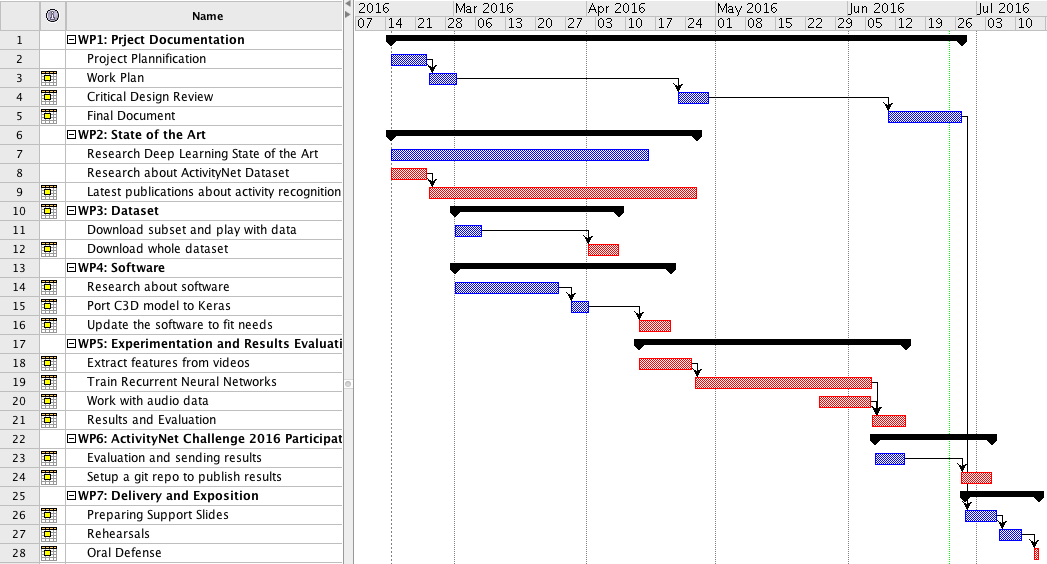
\includegraphics[width=1\linewidth]{img/introduction/gantt_diagram}
\end{center}
\caption{Gantt diagram of this thesis.}
\label{fig:gantt_diagram}
\end{figure}

\section{Work Plan Deviations and Incidents}
\label{section:work_plan_deviations}

The initial plan was to use the C3D\cite{tran2014learning} network to work with the video dataset which is based on the \textit{Caffe} deep learning framework. But in order to use Recurrent Neural Networks, \textit{Keras} was the best framework to use, so it was necessary to port the original model from one framework to the other.

Another deviation for the plan has been that, due to the huge amount of required computational resources, fine tuning the full C3D network has not been possible. Instead, the C3D framework has been used to extract features from the videos, which were then used as inputs to train the recurrent model to both classify and localize activities in videos.
